% !TEX root = ../TUCthesis.tex
%************************************************
\chapter{Grundlagen}\label{ch:grundlagen}
%************************************************

\ac{MtG} ist ein strategisches \ac{TCG}, bei dem zwei oder mehr Spieler mit einem individuellen Deck von Magic-Karten gegeneinander spielen. Im Laufe des Spiels werden verschiedene Karten, wie Länder, Kreaturen, Hexereien und andere Zauber eingesetzt, um das Spiel zu gewinnen \cite{rulebook:2013}. 

\section{Aufbau einer Karte}\label{ch:grundlagen:aufbau}
Die einfachste Möglichkeit Karten zu gruppieren ist anhand ihrer Farbe. Es gibt 5 verschiedene Farben in \ac{MtG}: \emph{weiß, blau, schwarz, grün} und \emph{rot} \cite{rulebook:2013}. Außerdem gibt es auch Karten die keiner Farbe angehören und daher als \emph{farblos} bezeichnet werden oder aber mehr als einer Farbe angehören, zum Beispiel gibt es Karten die sowohl \emph{rot} als auch \emph{grün} sind \cite{rulebook:2013}.

\subsection{Bestandteile einer Karte}

\begin{figure}[t]
	\myfloatalign
	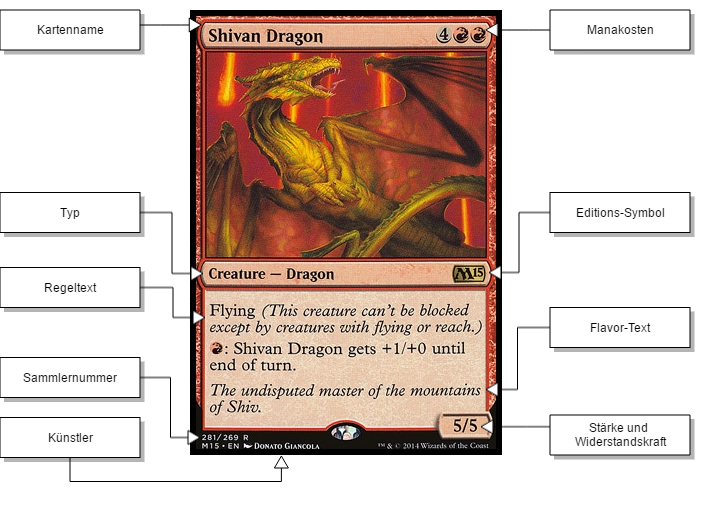
\includegraphics[width=\textwidth]{gfx/card.png}
	\caption{Bestandteile einer Karten}
	\label{fig:cardparts}
\end{figure}

\paragraph{Kartenname} 
Jede Karte hat einen eindeutigen Namen \cite{rulebook:2013}.

\paragraph{Typ}
Jede Karte hat einen bestimmten Typ. Außerdem kann eine Karte zusätzlich noch einen \emph{Subtyp/Untertyp} oder \emph{Supertyp} haben  \cite{rulebook:2013}. Zum Beispiel: Der \emph{Shivan Dragon} in \autoref{fig:cardparts} hat den Typ \emph{Kreatur} und als Untertyp \emph{Drache}.

\paragraph{Regeltext}
Enthält die \emph{Fähigkeiten} einer Karte, sofern vorhanden \cite{rulebook:2013}.

\paragraph{Flavor-Text}
Enthält Informationen über den Welt von \ac{MtG} und hat keinerlei Auswirkungen auf das Spielgeschehen \cite{rulebook:2013}.

\paragraph{Sammlernummer}
Hilft dabei die Karten einer Edition zu sortieren/organisieren  \cite{rulebook:2013}.

\paragraph{Künstler}
Der Künstler von dem das Bild für die Karte stammt  \cite{rulebook:2013}.

\paragraph{Stärke und Widerstandskraft}
Jede \emph{Kreatur} hat einen Wert für Stärke und Widerstandskraft. Die erste Zahl gibt die Stärke an und die zweite die Widerstandskraft  \cite{rulebook:2013}.

\paragraph{Editions-Symbol}
Gibt Auskunft über die Edition aus der die Karte stammt. Die Farbe des Symbols verrät die Seltenheit: schwarz für häufige, silbern für nicht ganz so häufige, golden für seltene und rot-orange für sagenhafte Karten \cite{rulebook:2013}.

\paragraph{Manakosten}
Die Hauptressource in \ac{MtG} ist \emph{Mana}, welches von \emph{Ländern} produziert und für das spielen von \emph{Zaubern} benötigt wird \cite{rulebook:2013}. 

\subsection{Kartentypen und Fähigkeiten}
Jede Karte in \ac{MtG} hat einen oder mehrere von den insgesamt sechs Typen \emph{(Land, Artefakt, Kreatur, Verzauberung, Planeswalker, Spontanzauber und Hexerei)}. An dem Kartentyp erkennt man wie sich die Karte verhält, das heißt wann man sie spielen kann und was danach mit ihr geschieht \cite{rulebook:2013}.

Viele Karten haben Texte, die sich auf das Spielgeschehen auswirken können, sogenannte Fähigkeiten. Aufgrund der großen Anzahl an Karten und der damit verbunden hohen Anzahl an verschiedenen Fähigkeiten werden diese in \emph{statische}, \emph{ausgelöste} und \emph{aktivierte Fähigkeiten} unterteilt \cite{rulebook:2013}.

\paragraph{Statische Fähigkeiten}
heißen so, da sie, solange sich die Karte im Spiel befindet, sich nicht verändern und konstant aktiv ist \cite{rulebook:2013}.

\paragraph{Ausgelöste Fähigkeiten}
sind Fähigkeiten, die durch ein bestimmtes Ereignis ausgelöst werden. Es gibt mehrere Formulierungen anhand derer man diese Art identifizieren kann. Die häufigsten sind \emph{wenn}, \emph{immer wenn} und \emph{zu} \cite{rulebook:2013}.

\paragraph{Aktivierte Fähigkeiten}
 erkennt man am Doppelpunkt. Sie werden in der Form \verb|[Kosten] : [Effekt]| angegeben, das heißt man muss etwas einsetzen, um die Fähigkeit zu aktivieren \cite{rulebook:2013}.

\paragraph{Schlüsselworte}
Fähigkeiten, die auf ein einzelnes Wort oder Satz gekürzt sind und eventuell einen Erinnerungstext haben, heißen \emph{Schlüsselwort-Fähigkeiten} \cite{rulebook:2013}. Meistens handelt es sich um \emph{statische Fähigkeiten}, aber \emph{ausgelöste} und \emph{aktivierte Fähigkeiten} sind auch möglich \cite{rulebook:2013}.

\section{Aufbau eines Decks}\label{ch:grundlagen:deck}
Ein Deck muss aus mindestens 60 Karten bestehen, wobei nach oben hin keine Grenzen gesetzt sind \cite{rulebook:2013}. Aus strategischer Sicht ist es aber sinnvoll möglichst nicht mehr als 60 Karten zu verwenden, da sonst die Wahrscheinlichkeit sinkt, die passende Karte zu ziehen. Des Weiteren ist es verboten mehr als vier Exemplare einer Karte im Deck zu haben, mit Ausnahme von Standardland-Karten, welche beliebig oft im Deck sein dürfen \cite{rulebook:2013}. Daraus ergeben sich folgende Richtlinien: 
\begin{itemize}
    \item Ein Deck sollte zwischen 35\% und 40\% aus Ländern bestehen  \cite{wotc:gameplay}
    \item Ein Deck sollte zwischen 25\% und 40\% aus Kreaturen bestehen. Dabei sollte beachtet werden, dass die Manakosten gut verteilt sind  \cite{wotc:gameplay}
    \item Rest: Alles was nicht Land oder Kreatur ist und das Deck unterstützt \cite{wotc:gameplay}
\end{itemize}
Turniere bieten eine Besonderheit, da es hier verschiedene Formate gibt. Bei manchen sind fast alle Karten erlaubt wohingegen bei anderen Formaten nur Karte der letzten paar Jahre erlaubt sind \cite{wotc:gameplay}.

%\paragraph{Die Goldene Regel} Falls eine \ac{MtG} Karte dem Regelbuch widerspricht, hat die Karte Vorrang \cite{rulebook:2013}.  

\subsection{Deck-Typen}
Durch die große Menge an Karten und die goldene Regel \emph{(falls eine Karte dem Regelbuch widerspricht, hat die Karte Vorrang)} ergeben sich viele verschiedene Spielweisen und Strategien nach denen man sein Deck ausrichten kann. Dadurch entstehen einige Decktypen, die die oben genannten Richtlinien für ihre Strategie anpassen \cite{wotc:gameplay}. Decks die eine ähnliche Strategie haben oder gleich aufgebaut sind, werden unter einem Deck-Typ zusammengefasst \cite{haumagic}. Besonders starke Deck-Typen entstehen häufig durch die Analyse der einzelnen Karten und den Ergebnissen eines Decks in Turnieren \cite{haumagic}. Ein wichtiger Begriff ist hierbei die sogenannte Manakurve. Sie gibt an wie ausgewogen die Manakosten in einem Deck sind: eine "hohe Manakurve" bedeutet, dass das Deck viele teurer Karten hat, wohingegen eine "niedrige Manakurve" bedeutet, dass viele günstige Karten enthalten sind. 

\paragraph{Aggro}
Bei der Aggro-Strategie geht es darum den Gegner möglichst früh mit den eigenen Kreaturen zu überrennen \cite{wotc:gameplay}. Es wird durch die eigenen Kreaturen möglichst früh Druck auf den Gegner ausgeübt, um ihn so in die Verteidigung zu bringen \cite{wotc:gameplay}. Entscheidend für die Strategie sind eine geringe Manakurve und viele kleine Kreaturen.

\paragraph{Control}
Die Control-Strategie ist das genaue Gegenteil der Aggro-Strategie. Ziel ist es den Gegner solange in seiner Strategie zu stören, bis man im späten Spielverlauf die Partie mit eigenen wenigen starken Kreaturen das Spiel dominieren kann \cite{wotc:gameplay}. Kontrolldecks setzten in erster Linie auf defensive Zauberkarten, um den Gegner zu stören, und wenige teure Kreaturen, um damit das Spiel zu gewinnen \cite{wotc:gameplay}. 

\paragraph{Midrange}
Midrange-Decks sind eine Kombination aus Aggro- und Kontrolldecks. Sie sind sehr effizient und können sich an die Strategie des Gegners anpassen \cite{wotc:gameplay}. Anstatt sich auf eine Strategie festzulegen wechseln Midrange-Decks je nach Situation zwischen aggressiver und defensiver Spielweise \cite{wotc:gameplay}.

\paragraph{Kombo}
Kombo-Decks nutzen Synergien die aus dem Zusammenspiel mehrerer Karten ergeben \cite{wotc:gameplay}. Die Decks sind komplett darauf ausgerichtet, diese Synergien noch weiter zu unterstützen und dadurch die Oberhand in der Partie zu gewinnen \cite{wotc:gameplay}. Aufgrund der Vielzahl an Karten gibt es unendlich viele Karten-Kombinationen \cite{wotc:gameplay}.


\section{Turniere}
Turniere werden ähnlich wie beim Schach nach dem Schweizer System gespielt. Dies ist eine Variante des Rundensystem bei der die Teilnehmer jede Runde spielen und die Paarungen sich anhand der bisherigen Spiel-Ergebnisse ergeben \cite{starcitygames:swiss}. Dadurch wird sichergestellt, dass Spieler mit ähnlichen Ergebnissen gegeneinander antreten \cite{starcitygames:swiss}. Wie in \autoref{tab:swisspairings} zu sehen, ist die Anzahl der gespielten Runden nach der Anzahl der Teilnehmer gestaffelt. 

Eine Runde wird nach dem \emph{Best-of-Three} Modus gespielt, das heißt die Runde ist beendet, sobald ein Spieler 2 Spiele gewonnen hat. 

\begin{table}[t]
    \myfloatalign
    \caption{Anzahl der Runden die ab einer Teilnehmerzahl gespielt werden \cite{wotc:swiss}} 
    \begin{tabular}{cc|cc}
        \toprule 
        Spieler & Runden & Spieler & Runden \\ 
        \midrule 
        2      & 1 & 129-212   & 8  \\ 
        3-4    & 2 & 213-384   & 9  \\ 
        5-8    & 3 & 385-672   & 10 \\ 
        9-16   & 4 & 673-1248  & 11 \\ 
        17-32  & 5 & 1249-2272 & 12 \\ 
        33-64  & 6 & 2273+     & 13 \\ 
        64-128 & 7 &           &  \\ 
        \bottomrule 
    \end{tabular}
    \label{tab:swisspairings}
\end{table}

\subsection{Matchup}
Matchup ist ein Begriff, welcher aus der Deckanalyse stammt und die Gewinn- und Verlustchancen eines Decks gegen ein anderes beschreibt. Der Wert wird oft in Prozentangaben wie 60:40 angegeben oder auch einfach nur als schlechtes oder gutes Matchup.

\section{Graph-Datenbanken}
Ein Graph ist eine Sammlung von Objekten \emph{(Knoten)} und deren Verbindungen \emph{(Kanten)} \cite{robinsongraph:2015}. Graphen lassen sich vielfältig einsetzen, vom Straßennetz bis zur Krankengeschichte von Populationen \cite{robinsongraph:2015}. In \autoref{fig:simple_graph} sieht man eine einfache Unternehmenshierarchie als Graph dargestellt. 

\begin{figure}[h]
    \myfloatalign
    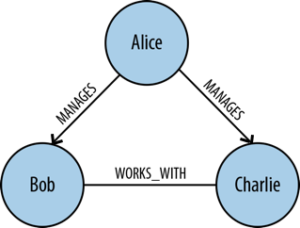
\includegraphics[width=0.65\textwidth]{gfx/simple_graph.png}
    \caption{Einfacher Graph \cite{neo4jblog:graph}}
    \label{fig:simple_graph}
\end{figure}

Ein \emph{Graph Datenbank Management System} (kurz \emph{Graph-Datenbank}) ist ein Datenbanken-Management-System, welches die \ac{CRUD} Eigenschaften unterstützt und ein Graph Daten-Modell bereitstellt \cite{robinsongraph:2015}.

Beziehungen in Graph-Datenbanken sind, im Gegensatz zu anderen Datenbank-Systemen, sogenannte \emph{first class citizens} \cite{robinsongraph:2015}. Dies bedeutet, dass Objekte mit einander verbunden werden können ohne dazu Fremdschlüssel oder ähnliche Konstrukte zu verwenden \cite{robinsongraph:2015}. Dadurch sind die Datenmodelle einfacher und ausdrucksvoller als Modelle von relationalen oder anderen \ac{NoSQL} Datenbanken \cite{robinsongraph:2015} .

\subsection{Stärken von Graph-Datenbanken}
Aufgrund der Tatsache, dass Abfragen nur auf einem Teil des Graphen arbeiten, bleibt die Performance einer Graph-Datenbank relativ konstant auch wenn der Datensatz wächst \cite{robinsongraph:2015}. Bei relationalen Datenbank Abfragen mit vielen \verb|JOIN|-Abfragen hingegen verschlechtert sich die Abfrageperformance bei zunehmenden Datensatz \cite{robinsongraph:2015}. 

Eine weitere Stärke von Graph-Datenbanken ist ihr flexibles Datenmodell. Es können neue Beziehungen, Knoten oder Untergraphen zu bestehenden Strukturen hinzugefügt werden ohne, dass es dabei zu Konflikten mit vorhandene Abfragen kommt \cite{robinsongraph:2015}. Dies bedeutet, dass das Datenmodell nicht ausführlich mit allen Details vor Projektbeginn vorhanden sein muss, sondern an geänderte Anforderungen im Laufe des Projekts angepasst werden kann \cite{robinsongraph:2015}. 
